\documentclass[tikz,border=3mm,multi=tikzpicture]{standalone}
\usepackage{tikz}
\usetikzlibrary{arrows.meta,positioning,calc}
\begin{document}

% TikZ 1
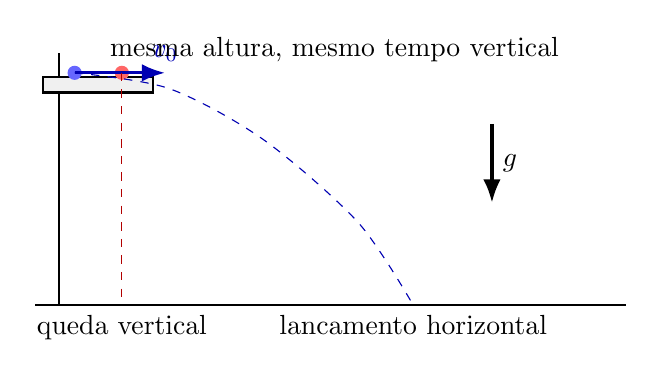
\begin{tikzpicture}[x=1cm,y=1cm,>=Latex]
  \draw[thick] (-0.3,0) -- (7.2,0);
  \draw[thick] (0,0) -- (0,3.2);
  \draw[thick,fill=gray!12] (-0.2,2.7) rectangle (1.2,2.9);
  \fill[blue!60] (0.2,2.95) circle (0.09);
  \fill[red!60] (0.8,2.95) circle (0.09);
  \draw[very thick,->,blue!70!black] (0.2,2.95) -- (1.35,2.95) node[above] {$v_0$};
  \draw[dashed,blue!70!black] plot[smooth] coordinates {(0.2,2.95) (1.4,2.75) (2.6,2.1) (3.8,1.05) (4.5,0)};
  \draw[dashed,red!70!black] (0.8,2.95) -- (0.8,0);
  \draw[->,very thick] (5.5,2.3) -- (5.5,1.3) node[midway,right] {$g$};
  \node[align=center] at (3.5,3.25) {mesma altura, mesmo tempo vertical};
  \node[below] at (0.8,0) {queda vertical};
  \node[below] at (4.5,0) {lancamento horizontal};
\end{tikzpicture}

% TikZ 2
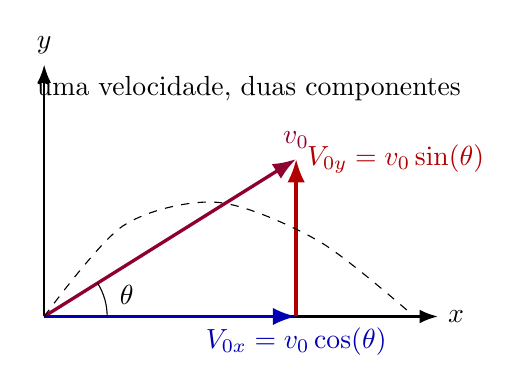
\begin{tikzpicture}[x=1cm,y=1cm,>=Latex]
  \draw[->,thick] (0,0) -- (5,0) node[right] {$x$};
  \draw[->,thick] (0,0) -- (0,3.2) node[above] {$y$};
  \draw[very thick,->,purple!75!black] (0,0) -- (3.2,2.0) node[above] {$v_0$};
  \draw[very thick,->,blue!70!black] (0,0) -- (3.2,0) node[below] {$V_{0x}=v_0\cos(\theta)$};
  \draw[very thick,->,red!70!black] (3.2,0) -- (3.2,2.0) node[right] {$V_{0y}=v_0\sin(\theta)$};
  \draw (0.8,0) arc[start angle=0,end angle=32,radius=0.8];
  \node at (1.05,0.28) {$\theta$};
  \draw[dashed] plot[smooth] coordinates {(0,0) (1,1.15) (2.2,1.45) (3.5,0.95) (4.7,0)};
  \node[align=center] at (2.6,2.9) {uma velocidade, duas componentes};
\end{tikzpicture}

\end{document}
